
\chapter{Testing and results}
\section{Testing the Code}
After testing the Code those are the results the we came to. 

 As we can see in the beginning  the process actively requests input from the user in order to proceed the implementation. it started by asking the user about his login credentials and then the Project ID that the user want to process, lastly before proceeding the creation and the command sending to XNAT, it asked the user about the command name and the description.
 After receiving  all the informations the script commence building the image, tagging, pushing, writing the JSON Command, enabling the Command, and lastly launch the container with all files.


 
 \section{Results on XNAT}
 The result that we came to after testing the code is that all the steps are working amazingly except that the container couldn't receive any files. with the \ac{STDout} view we found out that the Container received zero files. 
 
 \begin{figure}
    \centering
    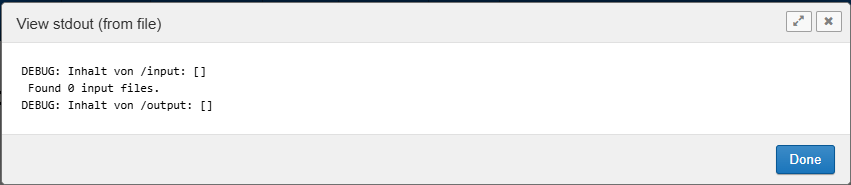
\includegraphics[width=0.9\textwidth]{en/content/STDOUT view.png}
    \caption{The STDout view of the Container on XNAT}
    \label{fig:enter-label}
\end{figure}

but weirdly after searching in the Container information, we noticed that the container in fact received the files and the file are listed in the input part of the container Input. 


\begin{figure}[p]
    \centering
    \rotatebox{90}{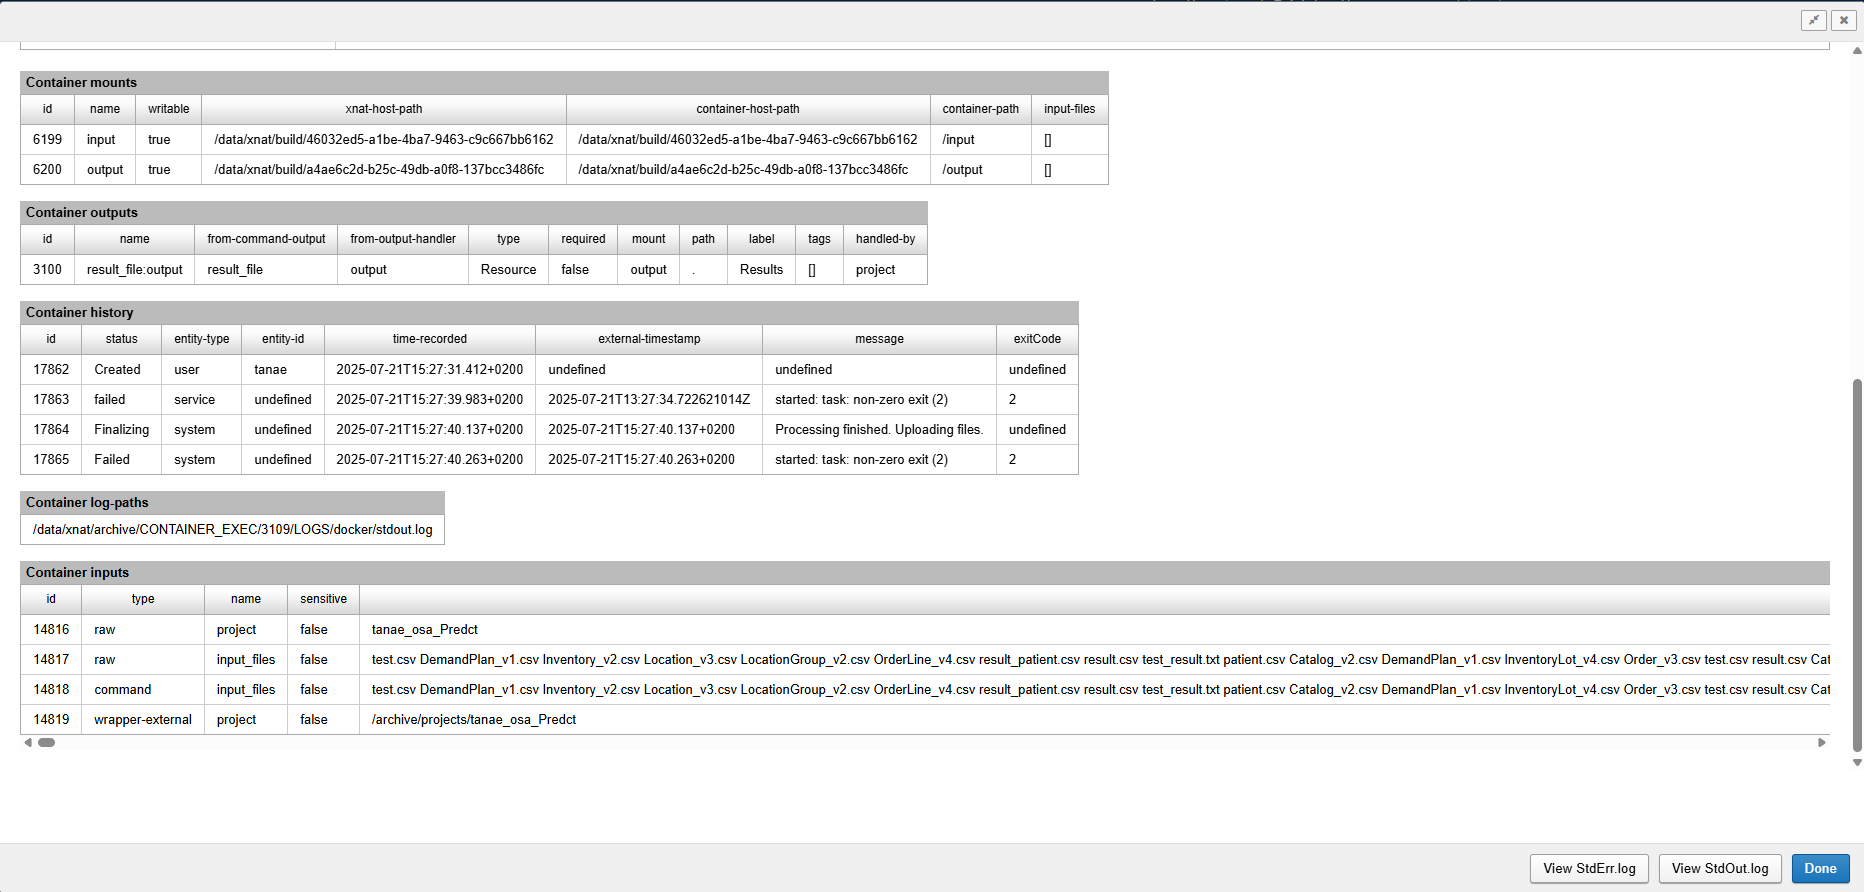
\includegraphics[width=0.95\textheight]{en/content/Container informatin 1.png}}
    \caption{Container Information 1}
    \label{fig:container-info-1}
\end{figure}


\begin{figure}
    \centering
    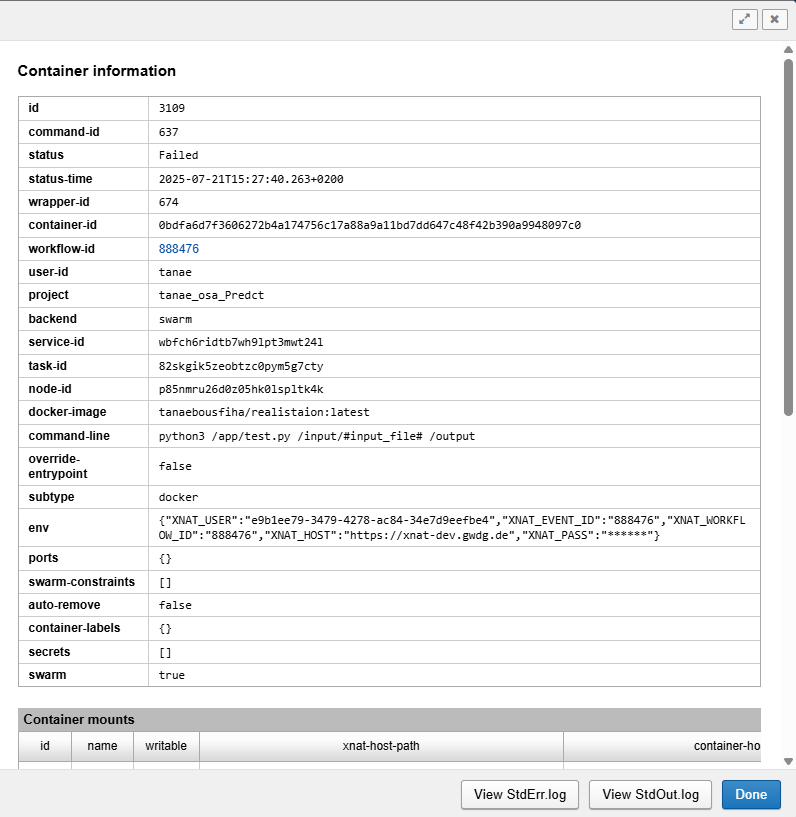
\includegraphics[width=0.9\linewidth]{en/content/Container information 2.png}
    \caption{Container Information 2 }
    \label{fig:enter-label}
\end{figure}

Details of the test procedure are described in Appendix A \cite{bousfiha2025appendix}..
.

The results demonstrate two things.  First, the automation script with the REST API worked correctly. Second, there is an issue with the container accessing the input files, despite them being listed as received.
